Die Signalverläufe geben Aufschluss über die Leitungskonstanten der Kabel. Wie in Kapitel \ref{seq:laplace} gezeigt, entstehen unterschiedliche Spannungsverläufe für unterschiedliche Ausgangsimpedanzen. Das geschlossene Kabel entspricht einer Induktivität und das offene Kabel einer Kapazität. Als Impedanz $Z_0$ ist für das vermessene Kabel ist
\begin{equation}
	Z_0 = \si{50}{\ohm}
\end{equation}
angegeben. Der Spannungsverlauf wird mit einem Oszilloskop aufgezeichnet und die Werte an den theoretischen Verlauf der Kurve gefittet. \
Aus den Parametern des Regression kann auch die Zeit bestimmt werden, die das Signal benötigt, bis das Ende des Kabels erreicht ist. Aus dieser Zeit wir am Ende des Kapitels die Länge des verwendeten Kabels bestimmt.

\subsubsection{Kabel mit geschlossenem Ende}
Der Signalverlauf ist in Abb. \ref{fig:oszi_geschlossen} dargestellt. Erwartet wird eine Flanke der Form
\begin{align}
			U(t) &= 2U_0\left(1 - \frac{Z_0}{R+Z_0} + \frac{Z_0}{R+Z_0}\exp\left(-\frac{R+Z_0}{L}t\right)\right) \\
			&= 2 a \left(1- b + b \exp(-c (t+d))   \right) + e \quad .
\end{align}
Es ist nur mit einer geeigneten Wahl der Startparameter möglich, einen guten Fit zu bekommen. Leider sind die so erhaltenen Abweichungen der Parameter dann unrealistisch und werden deswegen nicht weiter betrachtet. Die Funktion ist in Abb. \ref{fig:fit_geschlossen} dargestellt. Die verwendeten Parameter sind:
\begin{align}
	a &= \SI{-6.7339}{\volt}
 \\
	b &= \SI{0.9872}{}
 \\
	c &= \SI{0.0089}{\ohm\per\henry}
 \\
	d &= \SI{483.2099}{\nano\second}
 \\
	e &= \SI{12.5272}{\volt}
 
\end{align}
Aus den Parametern können der Widerstandsbelag $R$ und der Induktivitätsbelag $L$ des Kabels berechnet werden. Es muss beachtet werden, dass die Zeitskala Nanosekunden ist.
\begin{align}
	R &= \frac{Z_0}{b} - Z_0 = \SI{0.6507}{\ohm}
 \\
	L &= \frac{R + Z_0}{ c \cdot 10^9} = \SI{5.6828}{\micro\henry}

\end{align}



\begin{figure}
	\centering
	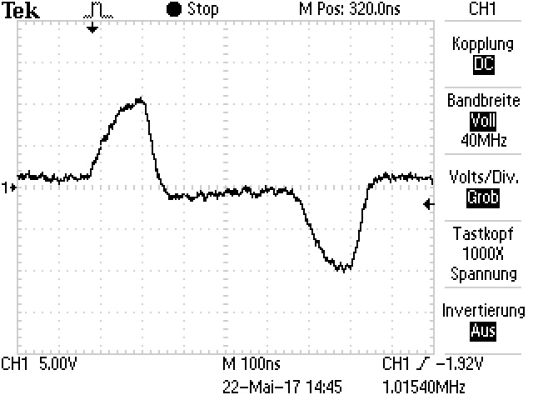
\includegraphics[width=0.7\textwidth]{Laplace/geschlossen.pdf}
\caption{Spannungsverlauf bei dem Kabel mit geschlossenem Ende}
\label{fig:oszi_geschlossen}
\end{figure}

\begin{figure}
	\centering
	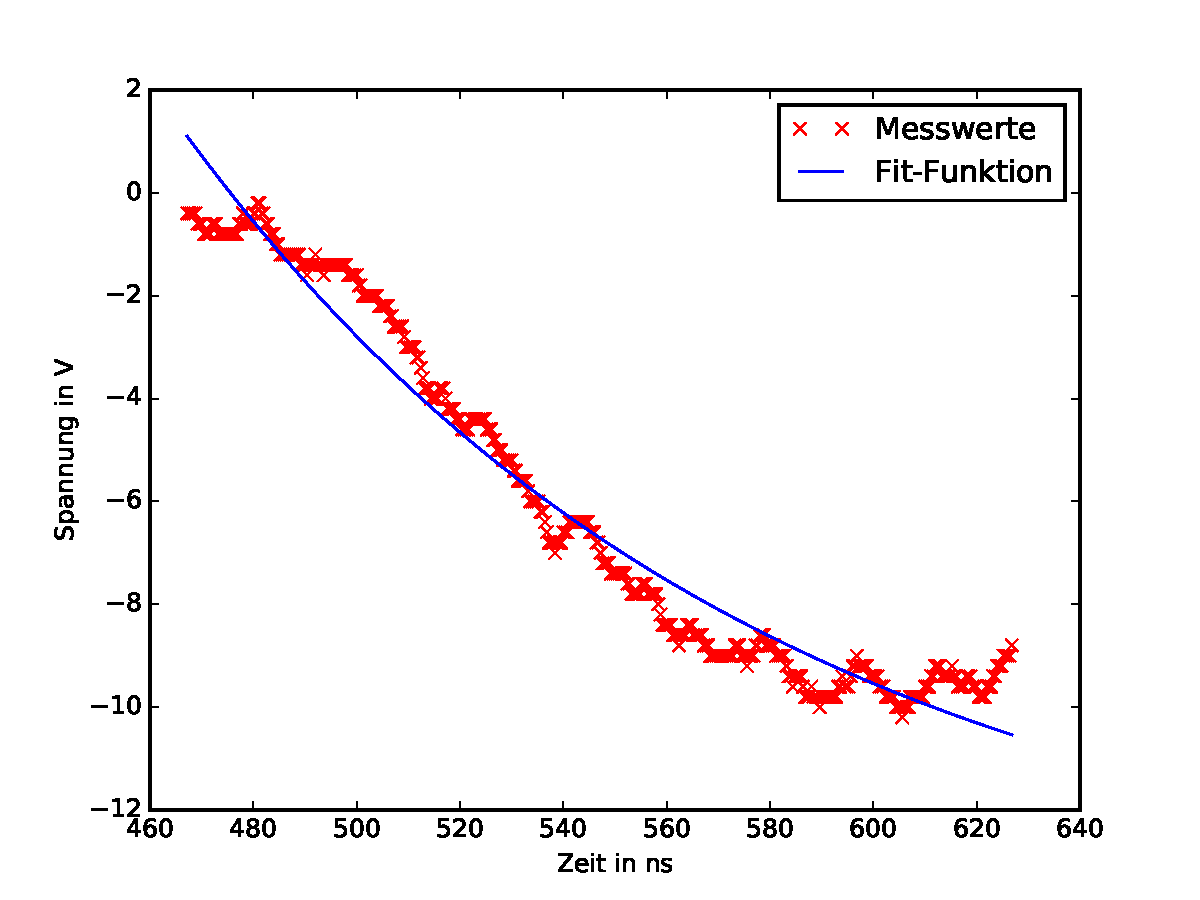
\includegraphics[width=0.7\textwidth]{Laplace/geschlossenes_ende.pdf}
	\caption{Fitfunktion an die fallende Flanke des Signalverlaufs bei dem Kabel mit geschlossenem Ende}
\label{fig:fit_geschlossen}
\end{figure}

\clearpage
\subsubsection{Kabel mit offenem Ende}
Der Spannungsverlauf des offenen Kabels ist in  Abb. \ref{fig:oszi_offen} zu sehen. Der Verlauf folgt der Funktionsvorschrift
\begin{align}
	U_0(t) &= 2U_0\left(1 -  \frac{Z_0}{R+Z_0} \exp \left( - \frac{1}{C(R+Z_0)} t\right) \right)\\
	&=  2 a (1 - b \exp(-c (x-d))) + e \quad .
\end{align}
Wie schon bei dem Kabel mit geschlossenem Ende müssen die Startwerte für die Parameter des Fits sehr exakt gewählt werden. Auch die ausgegebenen Abweichungen sind abermals nicht brauchbar. Der Plot ist in Abb. \ref{fig:fit_offen} dargestellt. Die Parameter sind:

\begin{align}
		a &= \SI{4.1028}{\volt}
 \\
		b &= \SI{0.6497}{}
 \\
		c &= \SI{0.0132}{\per\farad\per\ohm}
 \\
		d &= \SI{-466.8082}{\nano\second}
 \\
		e &= \SI{-10.8431}{\volt}
 
\end{align}
Es lassen sich die Kapazität $C$ des Kabels ebenso die der Widerstand $R$ aus den Parametern berechnen 
\begin{align}
	R &= \frac{Z_0}{b} - Z_0 = \SI{26.9529}{\ohm}
 \\
	C &= \frac{1}{ c (r + Z_0) \cdot 10^9} = \SI{985.9779}{\pico\farad}
 \quad.
\end{align}

\subsubsection{Kabellänge bestimmen}
\todo[color = red]{Haben wir für diese Messung das ganz lange Kabel benutzt? Die Werte sind so groß. Eigentlich hätte ich auch einen Faktor 2 in der Formel erwartet, aber in der Anleitung in Abb. 3 sieht das anders aus... }
Die Zeit~$T$ bis das Eingangssignal reflektiert wird ist gegeben durch 
\begin{equation}
	U_0(t) \propto \mathrm{e}^{-t/T} 
\end{equation}
und entspricht somit gerade dem Kehrwert des Fit-Parameters~$c$. Die Länge $l$ des Kabels lässt sich dann wie folgt berechnen
\begin{equation}
	l = T \cdot v = \frac{v}{c \cdot 10^{9}} \quad .
\end{equation}
Hierbei ist $v$ die Ausbreitungsgeschwindigkeit im Kabel, die gegeben ist durch
\begin{equation}
	v = \frac{c_{\textrm{Licht}}}{\sqrt{(\epsilon_r)}} = \frac{c_{\textrm{Licht}}}{\sqrt{(2.25)}} = \SI{199861638.7}{\meter\per\second}

\end{equation}
Da für in den Messungen mit dem offenen und dem geschlossenen Ende unterschiedliche Parameter $c$ gemessen wurden, obwohl es sich um das selbe Kabel handelt, werden die Längen einzeln ausgerechnet.
\begin{align}
	l_{\textrm{geschlossen}} &= \SI{22.4239}{\meter}
 \\
	l_{\textrm{offen}} &= \SI{15.1643}{\meter}

\end{align}

\clearpage

\begin{figure}
	\centering
	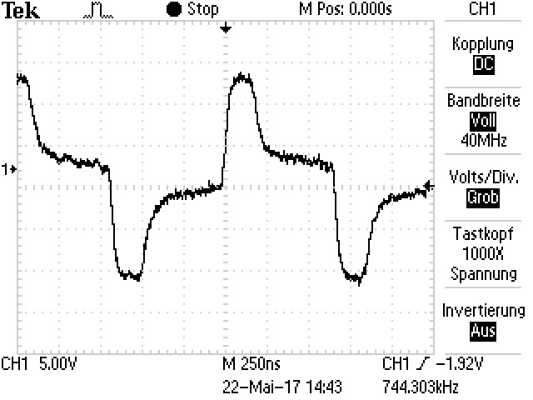
\includegraphics[width=0.7\textwidth]{Laplace/offen.pdf}
	\caption{Spannungsverlauf bei dem Kabel mit offenem Ende}
	\label{fig:oszi_offen}
\end{figure}

\begin{figure}
	\centering
	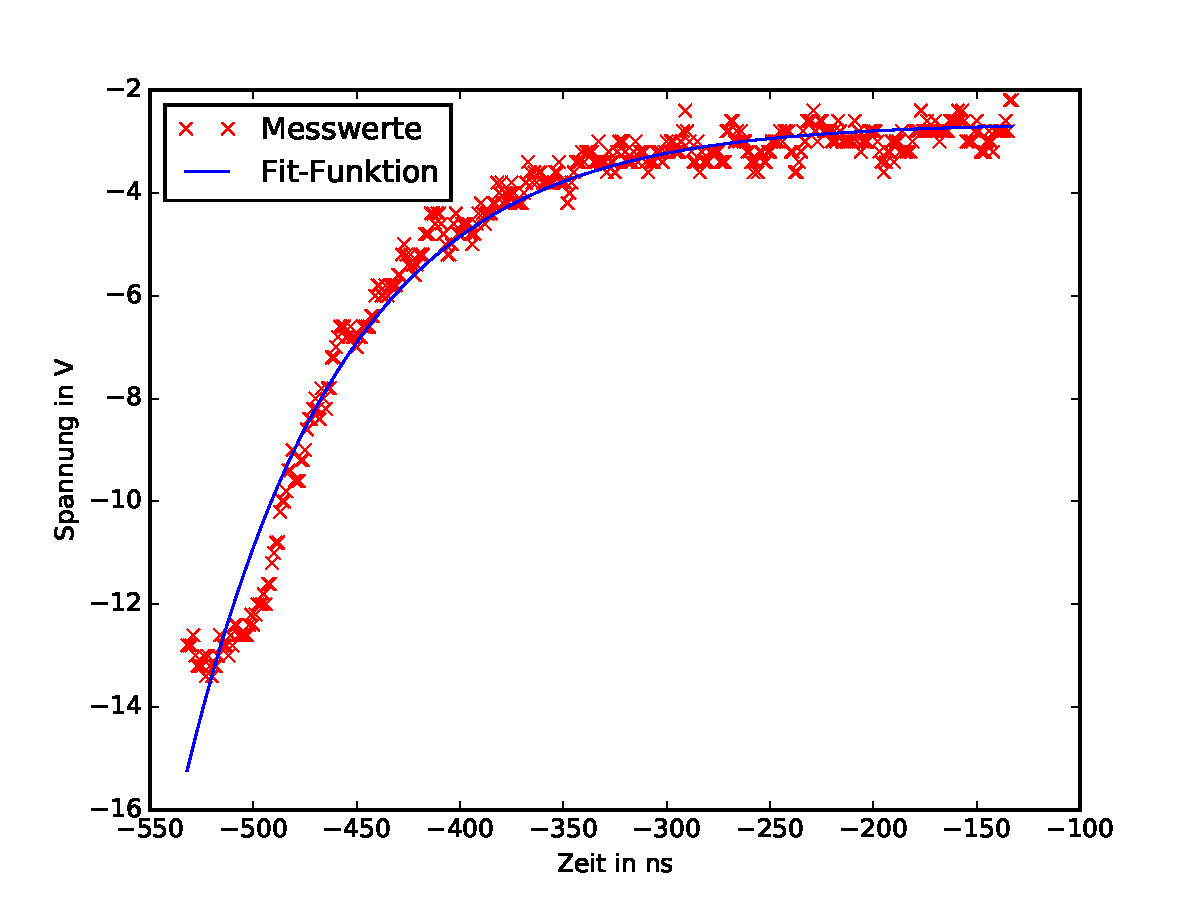
\includegraphics[width=0.7\textwidth]{Laplace/offenes_ende.pdf}
	\caption{Fitfunktion an die fallende Flanke des Signalverlaufs bei dem Kabel mit offenem Ende}
	\label{fig:fit_offen}
\end{figure}
